\documentclass{article}
\usepackage{tikz}
\usetikzlibrary{shapes,arrows}
\tikzstyle{block} = [draw, rectangle, minimum height=3em, minimum width=6em]
\tikzstyle{sum} = [draw, circle, node distance=1cm]
\tikzstyle{input} = [coordinate]
\tikzstyle{output} = [coordinate]
\tikzstyle{pinstyle} = [pin edge={to-,thin,black}]
\tikzstyle{vec->}=[line width=1mm,-stealth]
\tikzset{
	block/.style = {draw, fill=white, rectangle, minimum height=3em, minimum width=3em},
	%,
	tmp/.style  = {coordinate}, 
	sum/.style= {draw, fill=white, circle, node distance=1cm},
	input/.style = {coordinate},
	output/.style= {coordinate},
	pinstyle/.style = {pin edge={to-,thin,black}}
}

% Saturation block [satnode]
\pgfdeclareshape{satnode}{
\inheritsavedanchors[from={rectangle}]
\inheritbackgroundpath[from={rectangle}]
\inheritanchorborder[from={rectangle}]
\foreach \x in {center,north east,north west,north,south,south east,south west}{
\inheritanchor[from={rectangle}]{\x}
}
\foregroundpath{
\pgfpointdiff{\northeast}{\southwest}
\pgf@xa=\pgf@x \pgf@ya=\pgf@y
\northeast
\pgfpathmoveto{\pgfpoint{0}{0.45\pgf@ya}}
\pgfpathlineto{\pgfpoint{0}{-0.45\pgf@ya}}
\pgfpathmoveto{\pgfpoint{0.45\pgf@xa}{0}}
\pgfpathlineto{\pgfpoint{-0.45\pgf@xa}{0}}
\pgfpathmoveto{\pgfpointadd{\southwest}{\pgfpoint{-0.2\pgf@xa}{-0.3\pgf@ya}}}
\pgfpathlineto{\pgfpointadd{\southwest}{\pgfpoint{-0.5\pgf@xa}{-0.3\pgf@ya}}}
\pgfpathlineto{\pgfpointadd{\northeast}{\pgfpoint{-0.5\pgf@xa}{-0.3\pgf@ya}}}
\pgfpathlineto{\pgfpointadd{\northeast}{\pgfpoint{-0.2\pgf@xa}{-0.3\pgf@ya}}}
\pgfusepath{stroke}
}
}
\makeatother

\begin{document}

% The block diagram code is probably more verbose than necessary
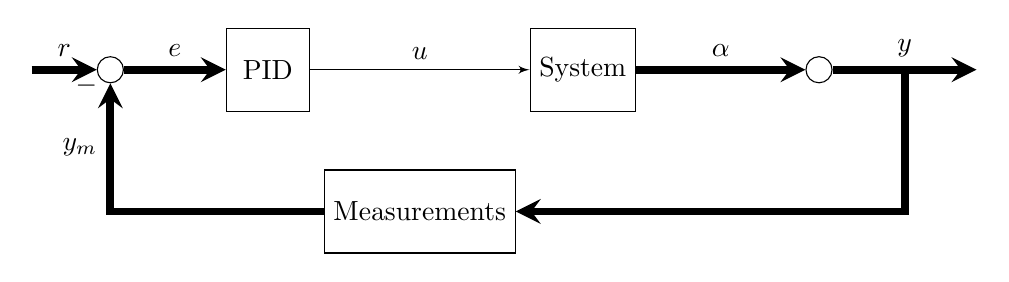
\begin{tikzpicture}[auto, node distance=2cm,>=latex']
    % We start by placing the blocks
    \node [input, name=input] {};
    \node [input, name=disturbance]{};
    \node [sum, right of=input] (sum) {};
    \node [block, right of=sum] (controller) {PID};
    \node [block, right of=controller, node distance=4cm] (system) {System};
    \node [sum, right of=system, node distance=3cm](sum2){};
    % We draw an edge between the controller and system block to 
    % calculate the coordinate u. We need it to place the measurement block. 
    \draw [->] (controller) -- node[name=u] {$u$} (system);
    \node [output, right of=sum2] (output) {};
    \node [block, below of=u] (measurements) {Measurements};

    % Once the nodes are placed, connecting them is easy. 
    \draw [draw,vec->] (input) -- node {$r$} (sum);
    \draw [vec->] (sum) -- node {$e$} (controller);
    \draw [vec->] (system) -- node{$\alpha$} (sum2);
    \draw [vec->] (sum2) -- node [name=y] {$y$}(output);
    \draw [vec->] (y) |- (measurements);
    \draw [vec->] (measurements) -| node[pos=0.99] {$-$} 
        node [near end] {$y_m$} (sum);
\end{tikzpicture}

\end{document}